%!TEX root = ../dissertation.tex
\chapter{Perspectives for molecular modeling}
\label{chap:appendix-a}

% \addcontentsline{toc}{*}{The future of molecular modeling}
\Lettrine{In} an ideal future, there would be no need for multiscale protocols because accuracy compromises will not be needed in exchange for performance. However, to get there a large series of milestones must be conquered first. That path can only be pursued if there is a global interest.

\section{The impact of molecular modeling}
%\addcontentsline{toc}{section}{The impact of molecular modeling}
\label{molecular-modeling-impact}

Such a vast array of tools and resources can only be product of thousands of researchers, both in the public and private sectors, and such devotion can only come if the field is attractive enough. Computational modeling is widely regarded as one of the fastest growing sectors in science, as perceived by researches and engineers themselves. According to a recent survey from the European FP7 project MULT-EU-SIM22, which measures the impact of general modeling in science and engineering, 75 $\%$  of researchers see a high impact of modeling and simulation in their fields, and 70 $\%$  foresee a strong growth of these methods, with an impact far beyond the currently achieved.\cite{ENN2012} International institutions also believe in the trend and, in fact, there are several ongoing projects working on standardizing basic concepts such as the terminology to be employed.\cite{cen2017} The very existence of reports covering the topic\cite{Goldbeck2012,Goldbeck2016,goldbeck2017} also serves as support for this general idea.

More concrete examples of this perception include the aerospace industry, which uses computational chemistry to better understand the effect of high temperatures and combustion on the stability of the coating present in the materials employed, thus increasing flight safety. Additionally, the longevity of nuclear reactors is affected by the impact of neutrons on the walls, which results in atomic displacement evaluable with computational chemistry. Better determining the life expectancy of the reactor and can potentially save millions by preventing an early shutdown of the plant.\cite{UKeconomics} In pharma, measuring the heat of formation experimentally is 50 times more expensive than a comparable DFT study.\cite{maginn2009}

These anecdotical examples can be quantified by analyzing some metrics on each of the three levels of the knowledge transmission model:\cite{warry2006} (1) Authors, (2) Users, (3) Society. The authors of theories and models (1), usually belonging to the academia, publish their findings to scientific journals, which end up in software products that can be used by professional modelers (2), leading to process improvements. This directly benefits society with lower prices in value products (3).

The increased popularity in basic research can be measured by the number of published manuscripts mentioning the topic, as well as their specific proportion within the field and impact factor. Observing the increasing presence of techniques such as DFT or molecular dynamics is a good proxy to the trend.\cite{maginn2009} An updated example can be seen in fig. \ref{fig:pubtrends}.


\begin{figure}[H]
	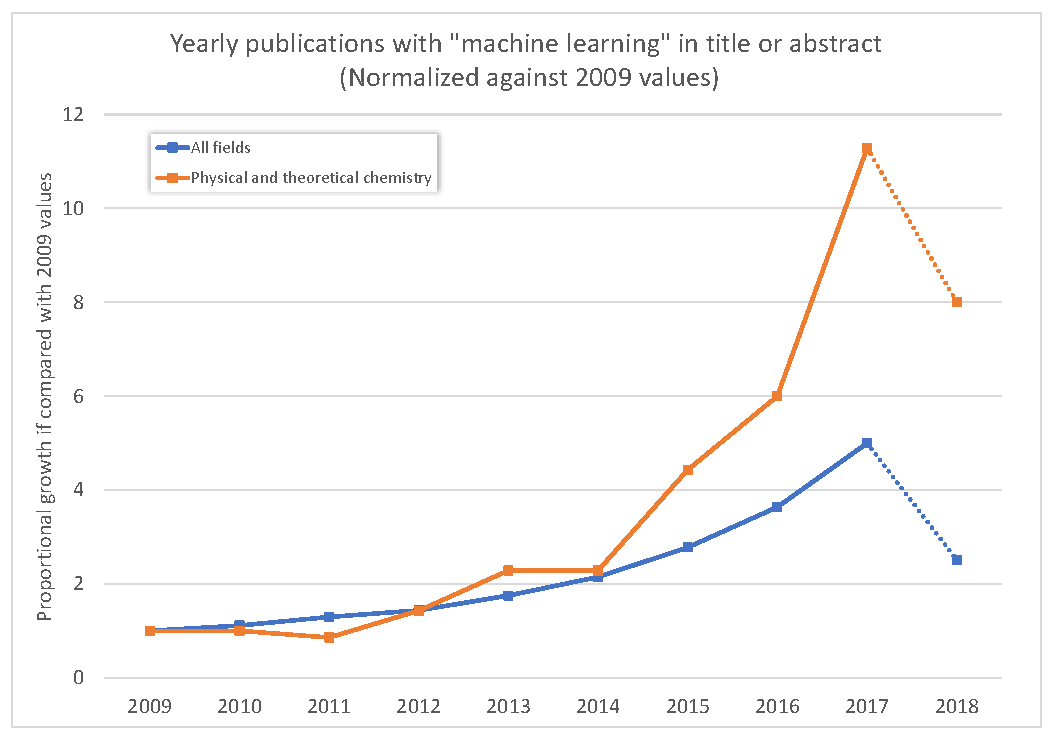
\includegraphics[width=\textwidth]{./figures/01/publication-trends_crop.pdf}
	\caption[Publication trends in molecular modeling]{Publication trends of manuscripts in molecular modeling in the title or abstract against all publications in chemistry related fields. Values are normalized against records in 2009. While publications in all chemistry exhibit a slower growth, articles in the field of molecular modeling (as represented with two popular methods, MD and DFT) have grown faster in the past decade. (Data obtained through \url{https://app.dimensions.ai}).}
	\label{fig:pubtrends}
\end{figure}


The direct application of methods is measurable by looking at the number of patents on the topic,\footnote{For example, at \url{http://www.wipo.int/patentscope}.} the return rate in the corresponding industries (between 3:1 and 10:1 in pharma\cite{accelryswhitepaper}), or the specific job postings demanding such experience.\footnote{Custom searches can be performed in websites such as \url{http://chemjobber.blogspot.com/}, \url{http://www.linkedin.com}, \url{http://glassdoor.com} or \url{http://www.stackoverflow.com}.}

In addition to the jobs themselves, which can be regarded as direct benefit for society, some other numbers could be thrown, such as the estimated contribution to the GDP by chemistry research (1.4$\%$  in UK as of 2010\cite{UKeconomics}), or the attributed spending on high performance computing by the modeling sectors, featuring bio-sciences, chemical engineering or computer-aided engineering as top contributors.\cite{hpc2020}

% \begin{itemize}
% 	\item \href{https://eic.rsc.org/feature/the-rise-of-molecular-modeling/3007610.article}{https://eic.rsc.org/feature/the-rise-of-molecular-modeling/3007610.article}

% 	\item \href{http://www.sciencedirect.com/science/article/pii/S1359644608001529}{http://www.sciencedirect.com/science/article/pii/S1359644608001529}
% \end{itemize}

\section{What the next generation will bring to the table}
% \addcontentsline{toc}{section}{What the next generation will bring to the table}

Published almost twenty years ago, the chapter \textit{Vision 2020: Computational Needs of the Chemical Industry} in \textit{Impact of Advances in Computing and Communications Technologies on Chemical Science and Technology: Report of a Workshop}\cite{vision2020} cited five main computational challenges for the chemical industry: Predicting (1) biological activity and (2) toxicity of a chemical structure, and designing (3) catalysts, (4) chemical processes and (5) materials. This englobes two intertwined areas: prediction and design. For this to happen, the report points that intense research must be carried out in, amongst others, the potential functions of MM-based methods, long MD simulations for large ensembles (in the millisecond scale), quantum effects, solvent effects, solid state structure, and multiscale protocols (atomistic, micro-, meso-, and macroscopic). Most of the challenges are accuracy or scale related, so huge efforts must be invested to reach errors within 0.1-0.2 kcal/mol in thermochemistry or to design universal and polarizable force fields, to cite two examples. This is not only a matter of scientific software development, but also responsibility of computer architecture, operating systems and networks. Since a single processor can only go so fast, tera-, peta- and exascales can only be achieved with parallel scaling, both within the processor itself (multicore architectures) and across symmetric machines (nodes within a cluster). For this to work reliably, the report suggests that operating systems and networks must be designed with fault tolerance in mind: if a core or node fails, the whole ensemble might fail as well.

We are almost in 2020 now, and part of the predictions and demands have been fulfilled. Massively parallel architectures are now inevitably present and software has been slowly adapting to the new design paradigms. Any research group or company can get access to these resources thanks to the ubiquitous \textit{cloud}, which offer hardware solutions on demand. The so-called \textit{as a Service}  products (Software as a Service, Platform as a Service\ldots) allow per-usage payments without having to worry about maintenance or resource constraints. If a given simulation needs more storage, memory or calculation speed, more nodes can be added to the ensemble with a click. Platforms such as Amazon's AWS, Google's Cloud or Microsoft's Azure\footnote{\url{https://aws.amazon.com}, \url{https://cloud.google.com}, \url{https://azure.microsoft.com}, respectively.} provide the raw infrastructure, which can be configured by the researchers or employees themselves, but is more commonly setup by specialized companies devoted to this newly found market niche.

What this report did not anticipate was the advent of GPGPU (General Purpose computing on Graphical Processor Units) computing: the advances in 3D acceleration and desktop graphics cards proved to be a massively parallel architecture that could be exploited by software not related to games and visualization. Molecular dynamics simulations have seen a drastic performance increase thanks to this new paradigm, implemented in all major suites (Amber,\cite{amber} Charmm,\cite{brooks1983} Gromacs,\cite{gromacs} NAMD,\cite{namd} HTMD,\cite{htmd} AceMD,\cite{acemd} OpenMM\cite{openmm}\ldots) and is now possible to simulate hundreds of nanoseconds a day with a sub-1000$\$$  personal desktop, thus getting closer to the proposed millisecond-scale that, while not routinely common, is starting to hit journals more often.\cite{shaw2008anton,lane2013} Quantum mechanics could certainly benefit from GPU acceleration, but the offer is still reduced (BigDFT,\cite{genovese2011daubechies} TeraChem\cite{luehr2011dynamic}). The following years will probably see a mainstream presence of GPU-implemented QM methods.

This would be in agreement with the 2017 Grimme's computational chemistry wish list for the upcoming 25 years: (1) Development of robust and fast electronic structure methods with chemical accuracy for all conceivable chemical processes, all states (gas, liquid, solid), and all (even exotic) types of spectroscopies, (2) Seamless and automated multilevel modeling, including error estimates, (3) Routine treatments for many nuclear degrees of freedom and entropy, (4) Inclusion of solvation effects, (5) Prediction of molecular as well as macroscopic (bulk) properties, and (6) Automated approaches for finding new reactions. Warshel, in his 2014 Nobel Lecture, pointed to broader future directions, like using molecular modeling to fight drug resistance, grasp a deeper understanding of protein-protein interactions, truly rational enzyme design or developing molecular machines; for all of them, multiscale strategies will be necessary, he concluded.\cite{Warshel2014}

These predictions can be further extended with more specific wishes, like universal reactive force fields or cheap, large-scale QM methods, two trends that will inevitably close the gap between these traditionally divergent approaches. Faster architecture and software will possibly allow for more robust \textit{ab initio} protein structure and folding studies,\cite{Lee2017} and cheminformatics tools like (3D)QSAR will also see advances.\cite{Cherkasov2013} Also, thanks again to hardware advances originally intended for gaming, Virtual and Augmented Realities will become mainstream and that should also influence molecular modeling software, whose graphical interfaces, built around an interactive 3D viewer, will be certainly enriched. As a matter of fact, several suites already include preliminary support.\cite{chimerax} Together with mobile and web platforms, desktop software will surely evolve to new interface paradigms.

Finally, an increasingly debated topic is the incursion of machine learning and neural networks in scientific software. After gaining a huge popularity for successfully solving problems traditionally understood as \textit{easy for humans but hard for computers} (i.e. facial recognition, natural language interfaces, speech synthesis), it is now overflowing to fields like computational chemistry. Being such a hot topic, a lot of publications have arisen in the last years (see fig. \ref{fig:machinelearningtrends}). While some see these proposals as the definite solution to some chemistry problems like QSAR\cite{paliwal2015,Ma2015,schutt2016,goh2017,goh2017b,koutsoukas2017,mayr2016} or even DFT-trained electronic predictions,\cite{faber2017} a certain skepticism is also held by others,\cite{forbes4decades,benhenda} especially when it comes to the pharma industry and drug design.


\begin{figure}[H]
	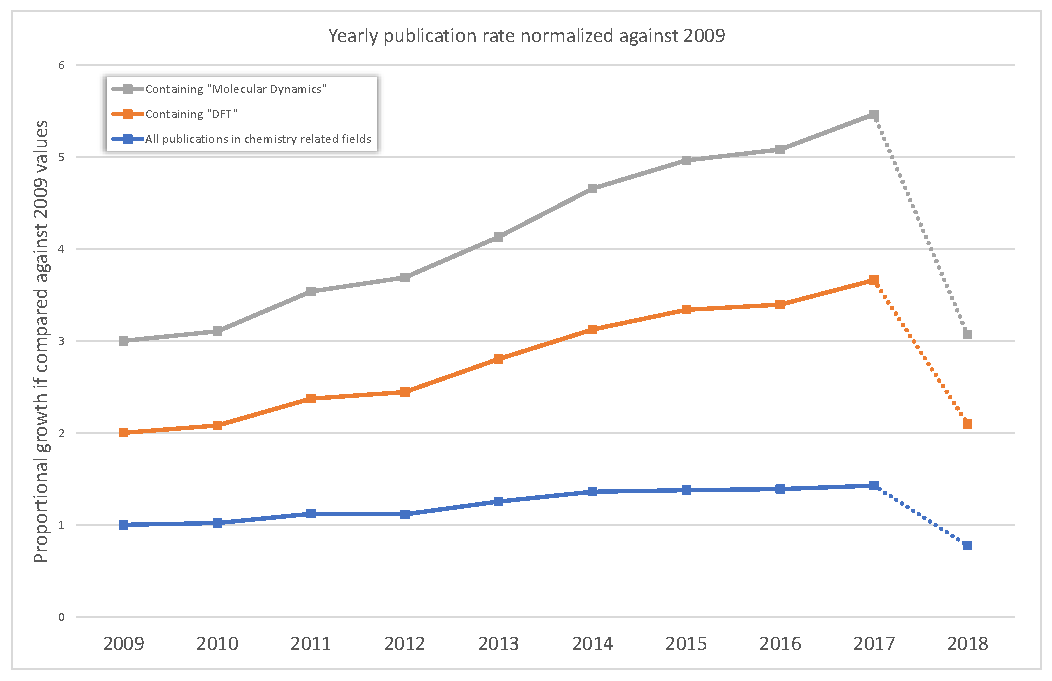
\includegraphics[width=\textwidth]{./figures/01/publication-trends-ml_crop.pdf}
	\caption[Machine learning publication trends]{Number of publications containing \textit{machine learning}  in title or abstract, per year. Data is normalized against the values recorded for 2009. Physical and theoretical chemistry exhibit a steeper growth in the recent years.}
	\label{fig:machinelearningtrends}
\end{figure}


Besides traditional computers, nascent quantum computing will be able to implement some algorithms with unprecedented efficiency. Computational chemistry will be one of the most benefitted fields in that regard,\cite{lanyon2010towards,zeng2017first,reiher2017elucidating} as prototyped in several recent attempts.\cite{hellweg2017brick,kandala2017hardware,sim2018quantum,dumitrescu2018cloud}

% Papers:

% \begin{itemize}
% 	\item \href{https://www.acs.org/content/acs/en/careers/college-to-career/chemistry-careers/computational-chemistry.html}{https://www.acs.org/content/acs/en/careers/college-to-career/chemistry-careers/computational-chemistry.html}

% 	\item \href{http://onlinelibrary.wiley.com/doi/10.1002/anie.201709943/full}{http://onlinelibrary.wiley.com/doi/10.1002/anie.201709943/full}

% 	\item \href{https://www.sciencedirect.com/science/article/pii/S0166354215300152}{https://www.sciencedirect.com/science/article/pii/S0166354215300152}

% Reading:

% 	\item \href{https://hub.wiley.com/community/exchanges/discover/blog/2014/02/05/a-day-in-the-life-of-a-computational-chemist}{https://hub.wiley.com/community/exchanges/discover/blog/2014/02/05/a-day-in-the-life-of-a-computational-chemist}

% 	\item \href{http://sciencenordic.com/nanomedicines-future-will-build-quantum-chemistry}{http://sciencenordic.com/nanomedicines-future-will-build-quantum-chemistry}

% 	\item \href{https://medium.com/@ShaliniAnanda1/ai-and-the-future-of-computational-chemistry-220dc462e092}{https://medium.com/@ShaliniAnanda1/ai-and-the-future-of-computational-chemistry-220dc462e092}

% 	\item \href{https://mariobarbatti.wordpress.com/2013/12/15/is-there-a-fair-future-for-computational-theoretical-chemistry/}{https://mariobarbatti.wordpress.com/2013/12/15/is-there-a-fair-future-for-computational-theoretical-chemistry/}

% 	\item \href{https://www.researchgate.net/post/What\_is\_the\_future\_in\_computational\_Chemistry\_I\_really\_want\_to\_know\_because\_i\_am\_planing\_to\_do\_my\_PhD\_in\_the\_said\_field\_Ur\_suggestions\_wil\_hlp\_me}{https://www.researchgate.net/post/What\_is\_the\_future\_in\_computational\_Chemistry\_I\_really\_want\_to\_know\_because\_i\_am\_planing\_to\_do\_my\_PhD\_in\_the\_said\_field\_Ur\_suggestions\_wil\_hlp\_me}

% 	\item \href{https://www.reddit.com/r/chemistry/comments/5v8glr/what\_does\_the\_future\_of\_computational\_chemistry/}{https://www.reddit.com/r/chemistry/comments/5v8glr/what\_does\_the\_future\_of\_computational\_chemistry/}

% 	\item \href{https://www.quora.com/What-is-the-future-of-computational-chemistry}{https://www.quora.com/What-is-the-future-of-computational-chemistry}

% 	\item \href{https://news.ycombinator.com/item?id=12783673}{https://news.ycombinator.com/item?id=12783673}

% 	\item \href{http://blog.rguha.net/?p=1703}{http://blog.rguha.net/?p=1703}
% \end{itemize}
